\documentclass[aspectratio=169,10pt]{beamer}

\usepackage{iftex}
\ifPDFTeX
  \usepackage[utf8]{inputenc}
  \usepackage[T1]{fontenc}
  \usepackage{lmodern}
\else
  \usepackage{fontspec}
  \setmainfont{latinmodern-math.otf}[BoldFont=lmroman10-bold.otf, ItalicFont=lmroman10-italic.otf]
  \setsansfont{lmsans10-regular.otf}[BoldFont=lmsans10-bold.otf, ItalicFont=lmsans10-oblique.otf]
  \setmonofont{lmmono10-regular.otf}
\fi
\usepackage[spanish,es-noquoting,es-nodecimaldot]{babel}
\usepackage{booktabs}
\usepackage{graphicx}
\usepackage{xcolor}

\definecolor{utecblue}{HTML}{4C72B0}
\definecolor{control}{HTML}{4C72B0}
\definecolor{park}{HTML}{DD8452}
\definecolor{hunt}{HTML}{55A868}
\definecolor{als}{HTML}{C44E52}

\graphicspath{{figures/}{../../reports/figures/}}

\usetheme{default}
\usecolortheme{default}
\setbeamertemplate{navigation symbols}{}
\setbeamertemplate{itemize items}[circle]
\setbeamercolor{structure}{fg=utecblue}
\setbeamercolor{frametitle}{fg=structure}
\setbeamerfont{frametitle}{series=\bfseries,size=\large}
\setbeamertemplate{frametitle}{%
  \vspace{0.6em}\usebeamerfont{frametitle}\usebeamercolor[fg]{frametitle}\insertframetitle\par
  \vspace{-0.3em}{\color{structure}\rule{\textwidth}{0.6pt}}\par\vspace{0.2em}}
\setbeamertemplate{footline}{%
  \hfill\scriptsize\color{gray}\insertframenumber\hspace{1.5em}\vspace{0.8em}}

\title{\bfseries Dinámica de la marcha para la clasificación de enfermedades neurodegenerativas}
\subtitle{Modelado, evaluación y validación externa · Entrega P2}
\author{Luis Renato Alvarez Ccopa \quad Andersson Chiroque Silva \quad David Teofilo Orihuela Serafin \\[0.3em] Jeraldine Dione Rojas Vargas \quad Dayanna Gisell Quispe Gallardo}
\institute{Universidad de Ingeniería y Tecnología}
\date{Machine Learning · 2026-1}

\begin{document}

\begin{frame}[plain]
  \titlepage
\end{frame}

\begin{frame}{Problema y preguntas}
  Clasificación supervisada en cuatro clases a partir de cinco minutos de marcha instrumentada:
  \textbf{\color{control}control}, \textbf{\color{park}Parkinson (EP)}, \textbf{\color{hunt}Huntington (EH)} y \textbf{\color{als}ELA}.

  \vspace{0.8em}
  \begin{columns}[T]
    \begin{column}{0.48\textwidth}
      \textbf{Datos}
      \begin{itemize}
        \item \texttt{gaitndd}: 63 sujetos tras control de calidad, 14\,732 zancadas
        \item \texttt{gaitpdb}: 165 sujetos (EP y control), solo para validación externa
        \item Unidad de análisis: \textbf{el sujeto}
      \end{itemize}
    \end{column}
    \begin{column}{0.48\textwidth}
      \textbf{Preguntas de investigación}
      \begin{description}
        \item[PI1] ¿Distingue entre enfermedades o solo sano/enfermo?
        \item[PI2] ¿Cuánto infla evaluar ventanas? ¿Se pueden aprovechar sin fuga?
        \item[PI3] ¿Es patología o edad, sexo y velocidad?
      \end{description}
    \end{column}
  \end{columns}

  \vspace{0.8em}
  \begin{block}{Lo que dejó P1}
    Partición por sujeto obligatoria (la aleatoria infla de 0.62 a 0.81) · el filtrado cambia las conclusiones · controles 27 años más jóvenes que EP.
  \end{block}
\end{frame}

\begin{frame}{Recordatorio del análisis exploratorio}
  \centering
  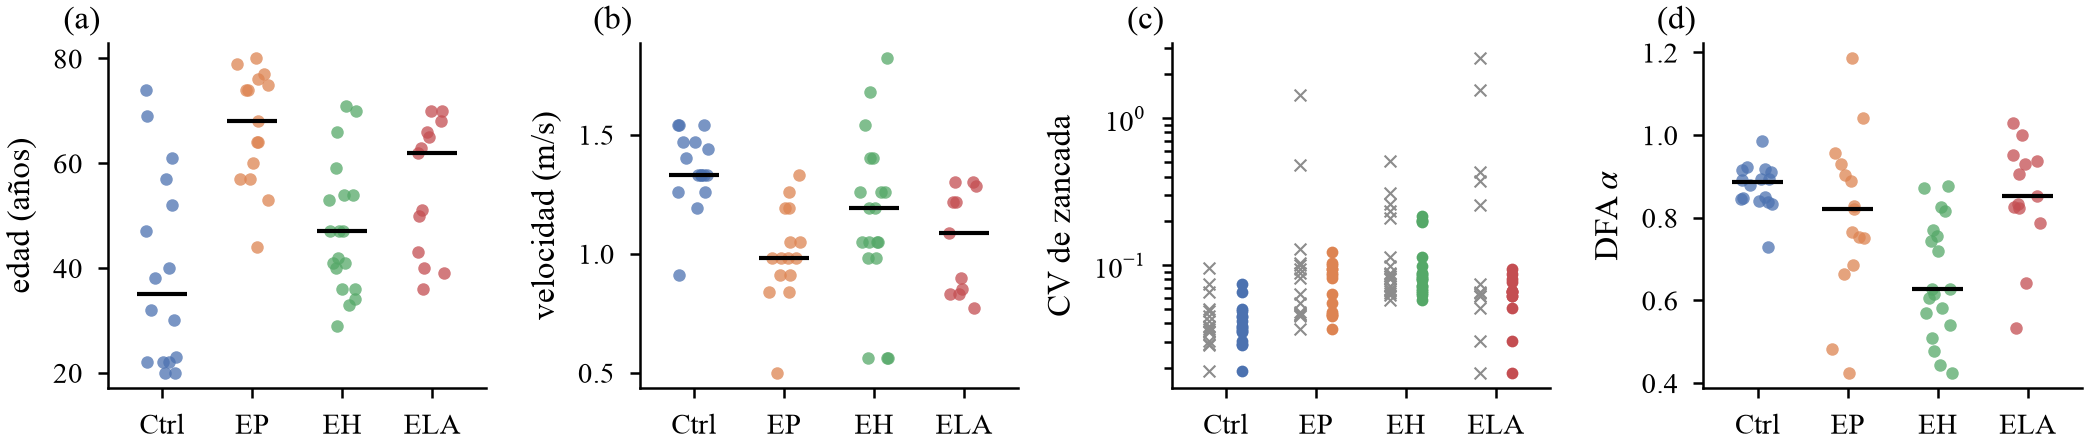
\includegraphics[width=\textwidth]{eda_resumen.png}

  \vspace{0.6em}
  \raggedright
  \small
  (a) edad y (b) velocidad difieren entre grupos: son confusores. (c) Sin filtrar, ELA parece la más variable; filtrado, lo es EH. (d) EH pierde memoria temporal (DFA $\alpha$ bajo). Ningún descriptor separa los cuatro grupos por sí solo.
\end{frame}

\begin{frame}{Preprocesamiento e ingeniería de características}
  \begin{columns}[T]
    \begin{column}{0.5\textwidth}
      \textbf{12 descriptores por sujeto}
      \begin{itemize}
        \item Ritmo: duración media
        \item Variabilidad: CV, IQR, \textbf{variabilidad sucesiva}
        \item Simetría: duración y balanceo
        \item Estructura temporal: autocorrelación, DFA $\alpha$, \textbf{entropía muestral}
        \item Fases: CV de balanceo, apoyo doble
      \end{itemize}
      \footnotesize En negrita, los nuevos de P2.
    \end{column}
    \begin{column}{0.48\textwidth}
      \textbf{Fuera del modelo}
      \begin{itemize}
        \item N.º de zancadas y cadencia: dependen del filtrado
        \item Balanceo medio: $r=-1.00$ con apoyo doble
        \item Severidad: fuga de la etiqueta
        \item Talla y peso: unidades inconsistentes
        \item Edad, sexo, velocidad: solo para estudiar confusores
      \end{itemize}
    \end{column}
  \end{columns}

  \vspace{0.8em}
  Imputación y escalamiento \textbf{dentro del pipeline}: se ajustan solo con los sujetos de entrenamiento de cada partición.
\end{frame}

\begin{frame}{Modelos y diseño experimental}
  \begin{columns}[T]
    \begin{column}{0.46\textwidth}
      \textbf{Referencias}
      \begin{itemize}
        \item Clase mayoritaria (azar = 0.25)
        \item Logística con CV y DFA, los dos marcadores clásicos
      \end{itemize}
      \vspace{0.4em}
      \textbf{Modelos} (12 descriptores)
      \begin{itemize}
        \item Regresión logística elastic net
        \item SVM con kernel RBF
        \item Bosque aleatorio
        \item Gradient boosting
        \item Logística y bosque \textbf{entrenados con ventanas}, decididos por sujeto
      \end{itemize}
    \end{column}
    \begin{column}{0.5\textwidth}
      \textbf{Validación cruzada anidada}
      \begin{itemize}
        \item Externa: 5 particiones $\times$ 10 repeticiones sobre sujetos
        \item Interna: búsqueda en grilla, 5 particiones agrupadas por sujeto
        \item Mismas 50 particiones para todos los modelos
      \end{itemize}
      \vspace{0.4em}
      \textbf{Métricas}: exactitud balanceada (principal), $F_1$ macro, AUC, sensibilidad por clase

      \vspace{0.4em}
      \textbf{Pruebas}: $t$ corregida de Nadeau--Bengio, permutación de etiquetas
    \end{column}
  \end{columns}
\end{frame}

\begin{frame}{Resultados: comparación de modelos}
  \begin{columns}[T]
    \begin{column}{0.5\textwidth}
      \centering
      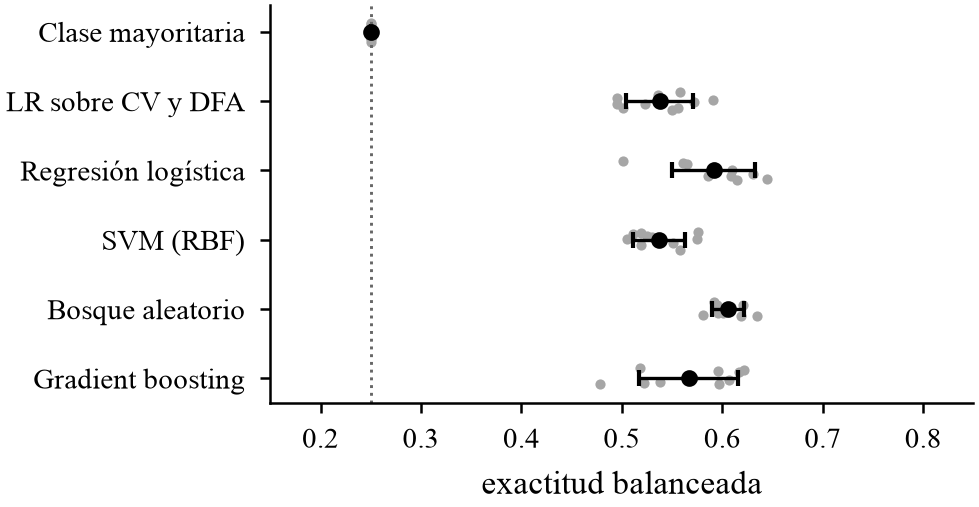
\includegraphics[width=\textwidth]{comparacion_modelos.png}
    \end{column}
    \begin{column}{0.48\textwidth}
      \small
      \begin{tabular}{lcc}
        \toprule
        Modelo & Exact. bal. & AUC \\
        \midrule
        Mayoritaria & 0.250 & 0.50 \\
        LR con CV y DFA & 0.538 & 0.74 \\
        Logística & 0.591 & 0.81 \\
        SVM & 0.537 & 0.78 \\
        \textbf{Bosque} & \textbf{0.605} & \textbf{0.83} \\
        Boosting & 0.566 & 0.76 \\
        \bottomrule
      \end{tabular}
    \end{column}
  \end{columns}

  \vspace{0.8em}
  \begin{itemize}
    \item Todos superan el azar (permutación: $p = 0.001$).
    \item \textbf{Ninguna diferencia entre modelos es significativa} (prueba $t$ corregida, $p > 0.2$): con 12--13 sujetos de prueba, un error mueve la partición en 0.08.
    \item EP es la clase más difícil en todos los modelos (sensibilidad 0.17--0.39).
  \end{itemize}
\end{frame}

\begin{frame}{PI2 · Entrenar con ventanas, decidir por sujeto}
  \centering
  \begin{tabular}{llc}
    \toprule
    Entrenamiento & Evaluación & Exactitud balanceada \\
    \midrule
    Ventanas, partición aleatoria (P1) & ventana & 0.812 \quad \textcolor{als}{fuga} \\
    Ventanas, partición agrupada (P1) & ventana & 0.622 \\
    \midrule
    Logística por sujeto & sujeto & 0.588 \\
    Logística por ventanas & sujeto & 0.641 \\
    Bosque por sujeto & sujeto & 0.613 \\
    \textbf{Bosque por ventanas} & sujeto & \textbf{0.647} \\
    \bottomrule
  \end{tabular}

  \vspace{1em}
  \raggedright
  \begin{itemize}
    \item Evaluar ventanas como independientes infla 19 puntos.
    \item Entrenar con ventanas y \textbf{promediar las probabilidades por sujeto} es válido: ningún sujeto de prueba tiene ventanas en el entrenamiento.
    \item Mejora de +0.04 a +0.05, pero no significativa ($p \approx 0.5$).
  \end{itemize}
\end{frame}

\begin{frame}{PI1 · ¿Distingue entre enfermedades?}
  \begin{columns}[T]
    \begin{column}{0.55\textwidth}
      \centering
      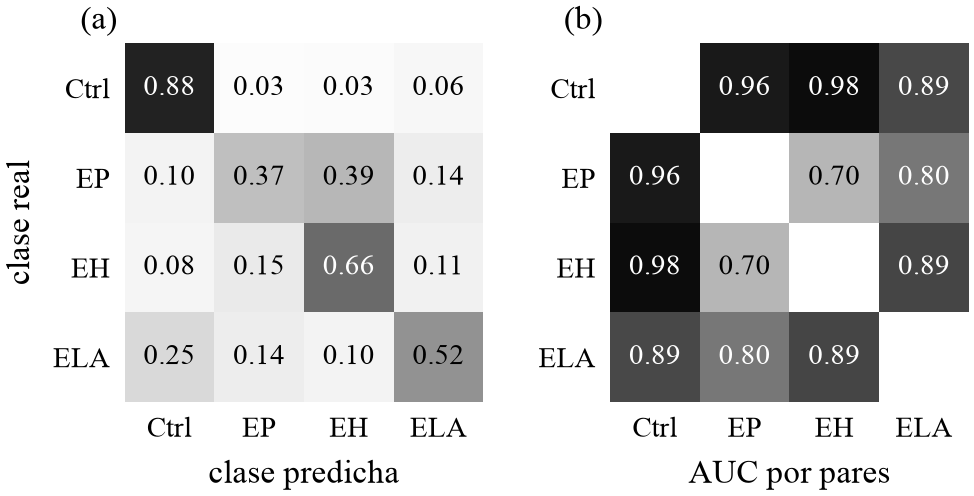
\includegraphics[width=\textwidth]{confusion_y_pares.png}

      \footnotesize (a) matriz de confusión del bosque; (b) AUC por pares
    \end{column}
    \begin{column}{0.43\textwidth}
      \small
      \begin{tabular}{lcc}
        \toprule
        Tarea & Azar & Exact. bal. \\
        \midrule
        Control vs.\ paciente & 0.50 & 0.86--0.87 \\
        EP / EH / ELA & 0.33 & 0.56--0.62 \\
        Cuatro clases & 0.25 & 0.59--0.61 \\
        \bottomrule
      \end{tabular}

      \vspace{0.8em}
      \begin{itemize}
        \item Sí distingue entre enfermedades, pero mucho menos que sano/enfermo.
        \item Par más difícil: \textbf{\color{park}EP}--\textbf{\color{hunt}EH} (AUC 0.70). El 39\,\% de los EP se predicen como EH.
      \end{itemize}
    \end{column}
  \end{columns}
\end{frame}

\begin{frame}{Análisis de errores: ¿a quién falla el modelo?}
  \centering
  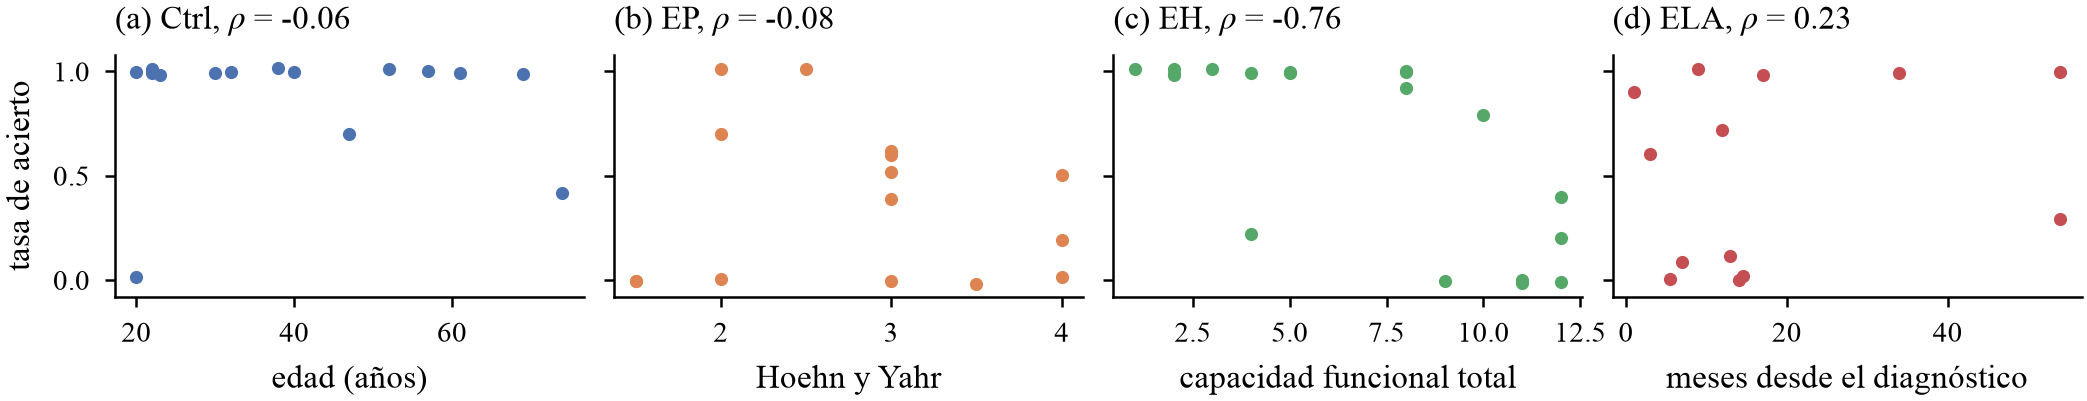
\includegraphics[width=\textwidth]{errores_severidad.png}

  \vspace{0.6em}
  \raggedright
  \begin{itemize}
    \item 29 sujetos se aciertan siempre y 14 se fallan en las 10 repeticiones.
    \item \textbf{\color{hunt}EH}: se fallan los \textbf{casos leves} (alta capacidad funcional, $\rho = -0.76$): su marcha todavía no es coreica.
    \item \textbf{\color{park}EP}: el más leve se confunde con control; los de alta variabilidad (CV 0.06--0.10) se confunden con EH.
    \item La severidad no entra al modelo (es fuga), solo se usa para explicar errores.
  \end{itemize}
\end{frame}

\begin{frame}{¿Qué usa el modelo? Importancia y confusores}
  \begin{columns}[T]
    \begin{column}{0.5\textwidth}
      \centering
      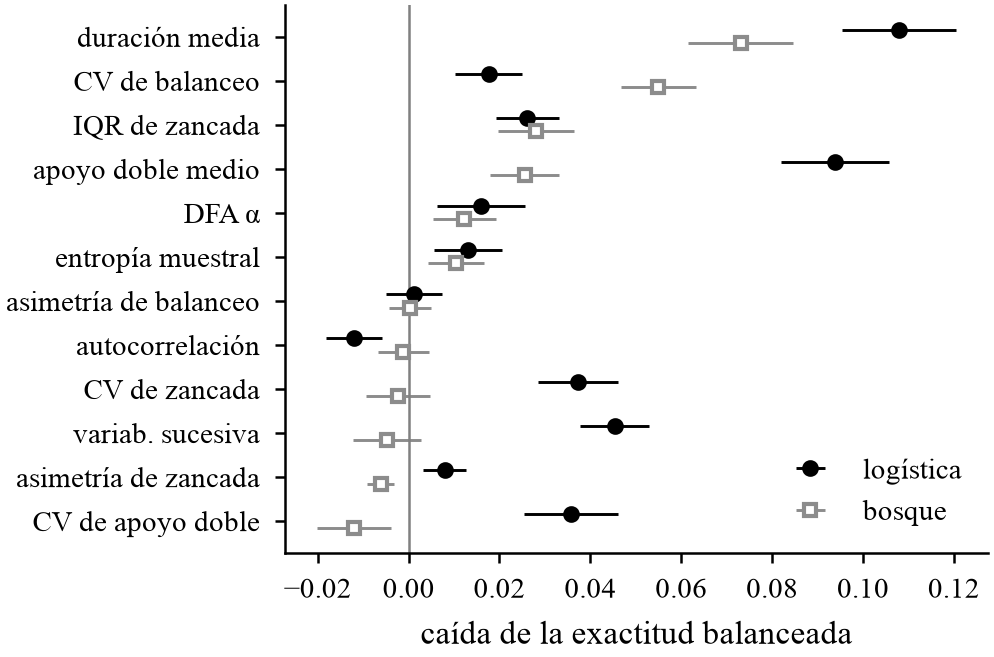
\includegraphics[width=\textwidth]{importancia_permutacion.png}
    \end{column}
    \begin{column}{0.48\textwidth}
      \small
      \textbf{Lo más importante: duración media de la zancada}, que depende de la velocidad.

      \vspace{0.6em}
      \begin{tabular}{lc}
        \toprule
        Variables & Exact. bal. \\
        \midrule
        Edad y sexo & 0.44--0.46 \\
        Velocidad & 0.40--0.52 \\
        Marcha & 0.59--0.61 \\
        Marcha + demografía & 0.66--0.68 \\
        \bottomrule
      \end{tabular}

      \vspace{0.6em}
      Dentro de \texttt{gaitndd}, la demografía ya separa los grupos: no se puede saber cuánto de la marcha es edad.
    \end{column}
  \end{columns}
\end{frame}

\begin{frame}{PI3 · Validación externa en \texttt{gaitpdb}}
  \begin{columns}[T]
    \begin{column}{0.36\textwidth}
      \centering
      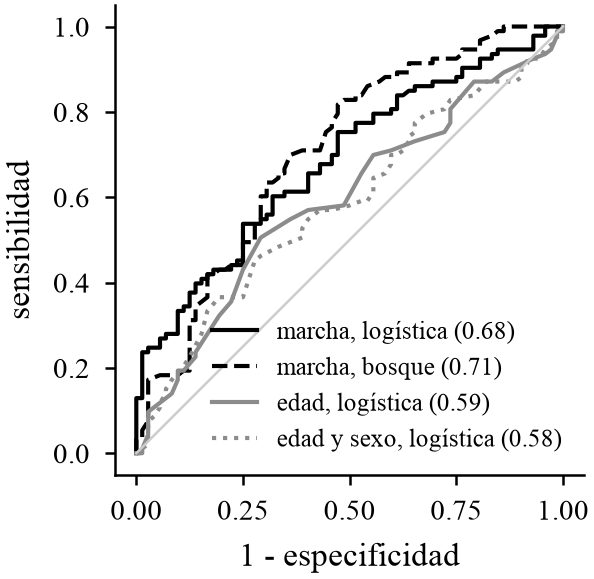
\includegraphics[width=\textwidth]{roc_externa.png}
    \end{column}
    \begin{column}{0.62\textwidth}
      Entrenado con 31 sujetos de \texttt{gaitndd} (EP vs.\ control) y aplicado \textbf{sin reentrenar} a 165 sujetos con edades comparables.

      \vspace{0.6em}
      \small
      \begin{tabular}{llcc}
        \toprule
        Variables & Modelo & AUC interna & AUC externa \\
        \midrule
        Tiempos de zancada & Bosque & 0.94 & \textbf{0.71} [0.63, 0.79] \\
        Tiempos de zancada & Logística & 0.81 & \textbf{0.68} [0.60, 0.76] \\
        Edad & Bosque & 0.74 & 0.52 [0.43, 0.61] \\
        Edad & Logística & 0.85 & 0.59 [0.51, 0.68] \\
        \bottomrule
      \end{tabular}

      \vspace{0.6em}
      \normalsize
      \begin{itemize}
        \item La edad pierde su capacidad; \textbf{la marcha la conserva}.
        \item Entrenando dentro de \texttt{gaitpdb}: AUC 0.69--0.71. El transporte casi no pierde.
        \item Umbral de contacto de 2 a 20\,\%: AUC entre 0.64 y 0.73.
      \end{itemize}
    \end{column}
  \end{columns}
\end{frame}

\begin{frame}{Lo que enseñó la versión preliminar con 19 descriptores}
  La primera versión usaba los 19 descriptores de P1, incluidos \textbf{n.º de zancadas, duración observada y cadencia}, con una sola validación cruzada.

  \vspace{0.8em}
  \begin{columns}[T]
    \begin{column}{0.48\textwidth}
      \textbf{Dentro de \texttt{gaitndd}}
      \begin{itemize}
        \item Una sola CV: DE entre particiones de 0.12--0.15; el 0.725 es un valor posible, pero promedia 0.628.
        \item Las 3 variables suben la logística de 0.618 a 0.668.
      \end{itemize}
    \end{column}
    \begin{column}{0.48\textwidth}
      \textbf{En \texttt{gaitpdb}}
      \begin{itemize}
        \item Zancadas: 250 vs.\ 103, \textbf{solo por durar 5 vs.\ 2 minutos}.
        \item Logística: predice EP en el 1.8\,\%; SVM, en el 100\,\%. Exactitud bal.\ 0.50.
        \item Sin esas 3 variables: 0.70.
      \end{itemize}
    \end{column}
  \end{columns}

  \vspace{1em}
  \begin{alertblock}{Una variable que describe el protocolo mejora la validación interna y rompe la externa}
    La validación cruzada no lo detecta porque todos los sujetos de una cohorte comparten protocolo.
  \end{alertblock}
\end{frame}

\begin{frame}{Limitaciones y consideraciones éticas}
  \begin{columns}[T]
    \begin{column}{0.5\textwidth}
      \textbf{Limitaciones}
      \begin{itemize}
        \item 13--19 sujetos por clase: diferencias de 0.05 no detectables.
        \item Edad y sexo siguen confundidos en \texttt{gaitndd}; solo EP--control tiene cohorte externa.
        \item Segmentación de \texttt{gaitpdb} sin eventos anotados a mano.
        \item Sin filtro el bosque rinde igual (0.611), pero usaría fallos del sensor como síntoma.
      \end{itemize}
    \end{column}
    \begin{column}{0.48\textwidth}
      \textbf{Ética}
      \begin{itemize}
        \item Datos públicos y anonimizados (ODC-By); no se redistribuyen.
        \item \textbf{No es una herramienta diagnóstica}: sensibilidad de 0.37 en EP.
        \item Cohortes pequeñas, de un centro, con sexo y edad desbalanceados: riesgo de peor desempeño en grupos no representados.
        \item La marcha revela estado de salud: exige consentimiento explícito.
      \end{itemize}
    \end{column}
  \end{columns}
\end{frame}

\begin{frame}{Conclusiones}
  \begin{description}
    \item[PI1] La marcha distingue entre enfermedades, pero mucho menos que sano/enfermo (0.56--0.62 frente a 0.86--0.87). La confusión principal es EP--EH.
      \vspace{0.4em}
    \item[PI2] Evaluar ventanas como independientes infla 19 puntos. Entrenar con ventanas y evaluar por sujeto da el mejor resultado: $0.647 \pm 0.028$.
      \vspace{0.4em}
    \item[PI3] En \texttt{gaitndd} edad y marcha no se pueden separar. En una cohorte con edades comparables, la marcha mantiene AUC 0.68--0.77 y la edad cae a 0.52--0.59.
  \end{description}

  \vspace{0.8em}
  \begin{block}{Aprendizaje principal}
    Con pocos sujetos, las decisiones de evaluación (unidad de partición, repeticiones, variables que dependen del protocolo) cambian el resultado más que pasar de un modelo lineal a un ensamble.
  \end{block}

  \vspace{0.4em}
  \small
  Trabajo futuro: cohortes externas para EH y ELA, adaptación de dominio entre sensores, regresión de severidad (UPDRS) y modelos sobre la señal cruda con más sujetos.
\end{frame}

\begin{frame}[plain]
  \vfill
  \centering
  {\Large\bfseries\color{structure} Gracias}

  \vspace{1.5em}
  \begin{tabular}{rl}
    Datos & PhysioNet \texttt{gaitndd} y \texttt{gaitpdb} (ODC-By 1.0) \\
    Código & \url{github.com/jeraldinedione/proyecto-machine-learning} \\
  \end{tabular}
  \vfill
\end{frame}

\end{document}
